% Generated by Sphinx.
\def\sphinxdocclass{report}
\documentclass[letterpaper,10pt,english]{sphinxmanual}
\usepackage[utf8]{inputenc}
\DeclareUnicodeCharacter{00A0}{\nobreakspace}
\usepackage{cmap}
\usepackage[T1]{fontenc}
\usepackage{babel}
\usepackage{times}
\usepackage[Bjarne]{fncychap}
\usepackage{longtable}
\usepackage{sphinx}
\usepackage{multirow}


\title{IM Documentation}
\date{September 15, 2014}
\release{1.0.0}
\author{Miguel Caballer Fernandez}
\newcommand{\sphinxlogo}{}
\renewcommand{\releasename}{Release}
\makeindex

\makeatletter
\def\PYG@reset{\let\PYG@it=\relax \let\PYG@bf=\relax%
    \let\PYG@ul=\relax \let\PYG@tc=\relax%
    \let\PYG@bc=\relax \let\PYG@ff=\relax}
\def\PYG@tok#1{\csname PYG@tok@#1\endcsname}
\def\PYG@toks#1+{\ifx\relax#1\empty\else%
    \PYG@tok{#1}\expandafter\PYG@toks\fi}
\def\PYG@do#1{\PYG@bc{\PYG@tc{\PYG@ul{%
    \PYG@it{\PYG@bf{\PYG@ff{#1}}}}}}}
\def\PYG#1#2{\PYG@reset\PYG@toks#1+\relax+\PYG@do{#2}}

\expandafter\def\csname PYG@tok@gd\endcsname{\def\PYG@tc##1{\textcolor[rgb]{0.63,0.00,0.00}{##1}}}
\expandafter\def\csname PYG@tok@gu\endcsname{\let\PYG@bf=\textbf\def\PYG@tc##1{\textcolor[rgb]{0.50,0.00,0.50}{##1}}}
\expandafter\def\csname PYG@tok@gt\endcsname{\def\PYG@tc##1{\textcolor[rgb]{0.00,0.27,0.87}{##1}}}
\expandafter\def\csname PYG@tok@gs\endcsname{\let\PYG@bf=\textbf}
\expandafter\def\csname PYG@tok@gr\endcsname{\def\PYG@tc##1{\textcolor[rgb]{1.00,0.00,0.00}{##1}}}
\expandafter\def\csname PYG@tok@cm\endcsname{\let\PYG@it=\textit\def\PYG@tc##1{\textcolor[rgb]{0.25,0.50,0.56}{##1}}}
\expandafter\def\csname PYG@tok@vg\endcsname{\def\PYG@tc##1{\textcolor[rgb]{0.73,0.38,0.84}{##1}}}
\expandafter\def\csname PYG@tok@m\endcsname{\def\PYG@tc##1{\textcolor[rgb]{0.13,0.50,0.31}{##1}}}
\expandafter\def\csname PYG@tok@mh\endcsname{\def\PYG@tc##1{\textcolor[rgb]{0.13,0.50,0.31}{##1}}}
\expandafter\def\csname PYG@tok@cs\endcsname{\def\PYG@tc##1{\textcolor[rgb]{0.25,0.50,0.56}{##1}}\def\PYG@bc##1{\setlength{\fboxsep}{0pt}\colorbox[rgb]{1.00,0.94,0.94}{\strut ##1}}}
\expandafter\def\csname PYG@tok@ge\endcsname{\let\PYG@it=\textit}
\expandafter\def\csname PYG@tok@vc\endcsname{\def\PYG@tc##1{\textcolor[rgb]{0.73,0.38,0.84}{##1}}}
\expandafter\def\csname PYG@tok@il\endcsname{\def\PYG@tc##1{\textcolor[rgb]{0.13,0.50,0.31}{##1}}}
\expandafter\def\csname PYG@tok@go\endcsname{\def\PYG@tc##1{\textcolor[rgb]{0.20,0.20,0.20}{##1}}}
\expandafter\def\csname PYG@tok@cp\endcsname{\def\PYG@tc##1{\textcolor[rgb]{0.00,0.44,0.13}{##1}}}
\expandafter\def\csname PYG@tok@gi\endcsname{\def\PYG@tc##1{\textcolor[rgb]{0.00,0.63,0.00}{##1}}}
\expandafter\def\csname PYG@tok@gh\endcsname{\let\PYG@bf=\textbf\def\PYG@tc##1{\textcolor[rgb]{0.00,0.00,0.50}{##1}}}
\expandafter\def\csname PYG@tok@ni\endcsname{\let\PYG@bf=\textbf\def\PYG@tc##1{\textcolor[rgb]{0.84,0.33,0.22}{##1}}}
\expandafter\def\csname PYG@tok@nl\endcsname{\let\PYG@bf=\textbf\def\PYG@tc##1{\textcolor[rgb]{0.00,0.13,0.44}{##1}}}
\expandafter\def\csname PYG@tok@nn\endcsname{\let\PYG@bf=\textbf\def\PYG@tc##1{\textcolor[rgb]{0.05,0.52,0.71}{##1}}}
\expandafter\def\csname PYG@tok@no\endcsname{\def\PYG@tc##1{\textcolor[rgb]{0.38,0.68,0.84}{##1}}}
\expandafter\def\csname PYG@tok@na\endcsname{\def\PYG@tc##1{\textcolor[rgb]{0.25,0.44,0.63}{##1}}}
\expandafter\def\csname PYG@tok@nb\endcsname{\def\PYG@tc##1{\textcolor[rgb]{0.00,0.44,0.13}{##1}}}
\expandafter\def\csname PYG@tok@nc\endcsname{\let\PYG@bf=\textbf\def\PYG@tc##1{\textcolor[rgb]{0.05,0.52,0.71}{##1}}}
\expandafter\def\csname PYG@tok@nd\endcsname{\let\PYG@bf=\textbf\def\PYG@tc##1{\textcolor[rgb]{0.33,0.33,0.33}{##1}}}
\expandafter\def\csname PYG@tok@ne\endcsname{\def\PYG@tc##1{\textcolor[rgb]{0.00,0.44,0.13}{##1}}}
\expandafter\def\csname PYG@tok@nf\endcsname{\def\PYG@tc##1{\textcolor[rgb]{0.02,0.16,0.49}{##1}}}
\expandafter\def\csname PYG@tok@si\endcsname{\let\PYG@it=\textit\def\PYG@tc##1{\textcolor[rgb]{0.44,0.63,0.82}{##1}}}
\expandafter\def\csname PYG@tok@s2\endcsname{\def\PYG@tc##1{\textcolor[rgb]{0.25,0.44,0.63}{##1}}}
\expandafter\def\csname PYG@tok@vi\endcsname{\def\PYG@tc##1{\textcolor[rgb]{0.73,0.38,0.84}{##1}}}
\expandafter\def\csname PYG@tok@nt\endcsname{\let\PYG@bf=\textbf\def\PYG@tc##1{\textcolor[rgb]{0.02,0.16,0.45}{##1}}}
\expandafter\def\csname PYG@tok@nv\endcsname{\def\PYG@tc##1{\textcolor[rgb]{0.73,0.38,0.84}{##1}}}
\expandafter\def\csname PYG@tok@s1\endcsname{\def\PYG@tc##1{\textcolor[rgb]{0.25,0.44,0.63}{##1}}}
\expandafter\def\csname PYG@tok@gp\endcsname{\let\PYG@bf=\textbf\def\PYG@tc##1{\textcolor[rgb]{0.78,0.36,0.04}{##1}}}
\expandafter\def\csname PYG@tok@sh\endcsname{\def\PYG@tc##1{\textcolor[rgb]{0.25,0.44,0.63}{##1}}}
\expandafter\def\csname PYG@tok@ow\endcsname{\let\PYG@bf=\textbf\def\PYG@tc##1{\textcolor[rgb]{0.00,0.44,0.13}{##1}}}
\expandafter\def\csname PYG@tok@sx\endcsname{\def\PYG@tc##1{\textcolor[rgb]{0.78,0.36,0.04}{##1}}}
\expandafter\def\csname PYG@tok@bp\endcsname{\def\PYG@tc##1{\textcolor[rgb]{0.00,0.44,0.13}{##1}}}
\expandafter\def\csname PYG@tok@c1\endcsname{\let\PYG@it=\textit\def\PYG@tc##1{\textcolor[rgb]{0.25,0.50,0.56}{##1}}}
\expandafter\def\csname PYG@tok@kc\endcsname{\let\PYG@bf=\textbf\def\PYG@tc##1{\textcolor[rgb]{0.00,0.44,0.13}{##1}}}
\expandafter\def\csname PYG@tok@c\endcsname{\let\PYG@it=\textit\def\PYG@tc##1{\textcolor[rgb]{0.25,0.50,0.56}{##1}}}
\expandafter\def\csname PYG@tok@mf\endcsname{\def\PYG@tc##1{\textcolor[rgb]{0.13,0.50,0.31}{##1}}}
\expandafter\def\csname PYG@tok@err\endcsname{\def\PYG@bc##1{\setlength{\fboxsep}{0pt}\fcolorbox[rgb]{1.00,0.00,0.00}{1,1,1}{\strut ##1}}}
\expandafter\def\csname PYG@tok@kd\endcsname{\let\PYG@bf=\textbf\def\PYG@tc##1{\textcolor[rgb]{0.00,0.44,0.13}{##1}}}
\expandafter\def\csname PYG@tok@ss\endcsname{\def\PYG@tc##1{\textcolor[rgb]{0.32,0.47,0.09}{##1}}}
\expandafter\def\csname PYG@tok@sr\endcsname{\def\PYG@tc##1{\textcolor[rgb]{0.14,0.33,0.53}{##1}}}
\expandafter\def\csname PYG@tok@mo\endcsname{\def\PYG@tc##1{\textcolor[rgb]{0.13,0.50,0.31}{##1}}}
\expandafter\def\csname PYG@tok@mi\endcsname{\def\PYG@tc##1{\textcolor[rgb]{0.13,0.50,0.31}{##1}}}
\expandafter\def\csname PYG@tok@kn\endcsname{\let\PYG@bf=\textbf\def\PYG@tc##1{\textcolor[rgb]{0.00,0.44,0.13}{##1}}}
\expandafter\def\csname PYG@tok@o\endcsname{\def\PYG@tc##1{\textcolor[rgb]{0.40,0.40,0.40}{##1}}}
\expandafter\def\csname PYG@tok@kr\endcsname{\let\PYG@bf=\textbf\def\PYG@tc##1{\textcolor[rgb]{0.00,0.44,0.13}{##1}}}
\expandafter\def\csname PYG@tok@s\endcsname{\def\PYG@tc##1{\textcolor[rgb]{0.25,0.44,0.63}{##1}}}
\expandafter\def\csname PYG@tok@kp\endcsname{\def\PYG@tc##1{\textcolor[rgb]{0.00,0.44,0.13}{##1}}}
\expandafter\def\csname PYG@tok@w\endcsname{\def\PYG@tc##1{\textcolor[rgb]{0.73,0.73,0.73}{##1}}}
\expandafter\def\csname PYG@tok@kt\endcsname{\def\PYG@tc##1{\textcolor[rgb]{0.56,0.13,0.00}{##1}}}
\expandafter\def\csname PYG@tok@sc\endcsname{\def\PYG@tc##1{\textcolor[rgb]{0.25,0.44,0.63}{##1}}}
\expandafter\def\csname PYG@tok@sb\endcsname{\def\PYG@tc##1{\textcolor[rgb]{0.25,0.44,0.63}{##1}}}
\expandafter\def\csname PYG@tok@k\endcsname{\let\PYG@bf=\textbf\def\PYG@tc##1{\textcolor[rgb]{0.00,0.44,0.13}{##1}}}
\expandafter\def\csname PYG@tok@se\endcsname{\let\PYG@bf=\textbf\def\PYG@tc##1{\textcolor[rgb]{0.25,0.44,0.63}{##1}}}
\expandafter\def\csname PYG@tok@sd\endcsname{\let\PYG@it=\textit\def\PYG@tc##1{\textcolor[rgb]{0.25,0.44,0.63}{##1}}}

\def\PYGZbs{\char`\\}
\def\PYGZus{\char`\_}
\def\PYGZob{\char`\{}
\def\PYGZcb{\char`\}}
\def\PYGZca{\char`\^}
\def\PYGZam{\char`\&}
\def\PYGZlt{\char`\<}
\def\PYGZgt{\char`\>}
\def\PYGZsh{\char`\#}
\def\PYGZpc{\char`\%}
\def\PYGZdl{\char`\$}
\def\PYGZhy{\char`\-}
\def\PYGZsq{\char`\'}
\def\PYGZdq{\char`\"}
\def\PYGZti{\char`\~}
% for compatibility with earlier versions
\def\PYGZat{@}
\def\PYGZlb{[}
\def\PYGZrb{]}
\makeatother

\begin{document}

\maketitle
\tableofcontents
\phantomsection\label{index::doc}


Contents:


\chapter{About IM}
\label{intro::doc}\label{intro:welcome-to-im-s-documentation}\label{intro:about-im}
Cloud infrastructures are becoming an appropriate solution to address the
computational needs of scientific applications. However, the use of public or
on-premises Infrastructure as a Service (IaaS) clouds require users to have
non-trivial system administration skills.

For that, IM is a \textbf{tool that ease the access and the usability of IaaS
clouds} by automating the VMI selection, deployment, configuration, software
installation, monitoring and update of Virtual Appliances. \textbf{It supports APIs
from a large number of virtual platforms}, making user applications
cloud-agnostic. In addition \textbf{it integrates a contextualization system} to
enable the installation and configuration of all the user required applications
providing the user with a fully functional infrastructure.

It is a service that features a \textbf{web-based GUI, a XML-RPC API, a REST API and
a command-line application}.


\chapter{IM Videos}
\label{videos::doc}\label{videos:im-videos}
There are an Infrastructure Manager youtube channel with a set of videos with demos
of the functionality of the platform.

Currently there are two videos available, but soon more videos will be uploaded:

The first one shows how to use the IM web interface to launch a Hadoop Cluster with a
single click in a OpenNebula on-premise cloud platform and in Amazon EC2.

The second video shows a demo of how to create a cluster with a single click using the
IM web interface with the EC3 tool. It also shows how CLUES works to dinamically manage
the size of the cluster automatically.

\href{https://www.youtube.com/channel/UCF16QmMHlRNtsC-0Cb2d8fg}{YouTube IM channel}


\chapter{IM Service Installation}
\label{manual::doc}\label{manual:im-service-installation}

\section{Prerequisites}
\label{manual:prerequisites}
IM needs at least Python 2.4 to run, as well as the next libraries:
\begin{itemize}
\item {} 
\href{http://www.dabeaz.com/ply/}{PLY}, Python Lex \& Yacc library for python.

\item {} 
\href{http://www.lag.net/paramiko/}{paramiko}, ssh2 protocol library for python.

\item {} 
\href{http://pyyaml.org/}{PyYAML}, a YAML parser.

\item {} 
\href{http://pywebsvcs.sourceforge.net/}{SOAPpy}, a full-featured SOAP library
(we know it is not actively supported by upstream anymore).

\end{itemize}

Also, IM uses \href{http://www.ansible.com}{Ansible} (1.4.2 or later) to configure the
infrastructure nodes.

These components are usually available from the distribution repositories. To
install them in Debian and Ubuntu based distributions, do:

\begin{Verbatim}[commandchars=\\\{\}]
\PYGZdl{} apt\PYGZhy{}get install python\PYGZhy{}ply python\PYGZhy{}paramiko python\PYGZhy{}yaml python\PYGZhy{}soappy ansible
\end{Verbatim}

In Red Hat based distributions (RHEL, CentOS, Amazon Linux, Oracle Linux,
Fedora, etc.), do:

\begin{Verbatim}[commandchars=\\\{\}]
\PYGZdl{} yum install python\PYGZhy{}ply python\PYGZhy{}paramiko PyYAML SOAPpy ansible
\end{Verbatim}

Finally, check the next values in the Ansible configuration file
\code{ansible.cfg}, (usually found in \code{/etc/ansible}):

\begin{Verbatim}[commandchars=\\\{\}]
\PYG{n}{host\PYGZus{}key\PYGZus{}checking} \PYG{o}{=} \PYG{n+nb+bp}{False}
\PYG{n}{transport} \PYG{o}{=} \PYG{n}{paramiko}
\PYG{n}{record\PYGZus{}host\PYGZus{}keys} \PYG{o}{=} \PYG{n+nb+bp}{False}
\end{Verbatim}


\section{Optional Packages}
\label{manual:optional-packages}\begin{itemize}
\item {} 
\href{http://libcloud.apache.org/}{apache-libcloud} 0.15 or later is used in the
LibCloud connector.

\item {} 
\href{http://boto.readthedocs.org}{boto} 2.19.0 or later is used as interface to
Amazon EC2. It is available as package named \code{python-boto} in Debian based
distributions. It can also be downloaded from \href{https://github.com/boto/boto}{boto GitHub repository}.
Download the file and copy the boto subdirectory into the IM install path.

\item {} 
\href{http://springpython.webfactional.com/}{Spring Python} framework is needed
if the access to XML-RPC API is secured with SSL certificates (see
{\hyperref[manual:confval-XMLRCP_SSL]{\code{XMLRCP\_SSL}}}).
The Debian package is named \code{python-springpython}.

\item {} 
\href{http://cherrypy.org}{CherryPy} is needed if needed to secure the REST API
with SSL certificates (see {\hyperref[manual:confval-REST_SSL]{\code{REST\_SSL}}}).
The Debian package is named \code{python-cherrypy3}.

\end{itemize}


\section{Installation}
\label{manual:installation}

\subsection{Form Pip}
\label{manual:form-pip}
You only have to call the install command of the pip tool with the IM package:

\begin{Verbatim}[commandchars=\\\{\}]
\PYGZdl{} pip install IM
\end{Verbatim}

\textbf{WARNING: In some linux distributions (REL 6 or equivalents) you must unistall
the packages python-paramiko and python-crypto before installing the IM with pip.}

Pip will install all the pre-requisites needed. So Ansible 1.4.2 or later will be
installed in the system. In some cases it will need to have installed the GCC
compiler and the python developer libraries (`python-dev' or `python-devel'
packages in main distributions).

You must also remember to modify the ansible.cfg file setting as specified in the
REQUISITES section.


\subsection{Form Source}
\label{manual:form-source}
Once the dependences are installed, just download the tarball of \emph{IM Service}
from \href{http://www.grycap.upv.es/im/download.php}{Download}, extract the
content and move the extracted directory to the installation path (for instance
\code{/usr/local} or \code{/opt}):

\begin{Verbatim}[commandchars=\\\{\}]
\PYGZdl{} tar xvzf IM\PYGZhy{}0.1.tar.gz
\PYGZdl{} sudo chown \PYGZhy{}R root:root IM\PYGZhy{}0.1.tar.gz
\PYGZdl{} sudo mv IM\PYGZhy{}0.1 /usr/local
\end{Verbatim}

Finally you must copy (or link) \$IM\_PATH/im file to /etc/init.d directory:

\begin{Verbatim}[commandchars=\\\{\}]
\PYGZdl{} sudo ln \PYGZhy{}s /usr/local/IM\PYGZhy{}0.1/im /etc/init.d
\end{Verbatim}


\section{Configuration}
\label{manual:configuration}
If you want the IM Service to be started at boot time, do
\begin{enumerate}
\item {} 
Update the value of the variable \code{IMDAEMON} in \code{/etc/init.d/im} file
to the path where the IM im\_service.py file is installed (e.g. /usr/local/im/im\_service.py),
or set the name of the script file (im\_service.py) if the file is in the PATH
(pip puts the im\_service.py file in the PATH as default):

\begin{Verbatim}[commandchars=\\\{\}]
\PYGZdl{} sudo sed \PYGZhy{}i \PYGZsq{}s/{}`IMDAEMON=.*/{}`IMDAEMON=/usr/local/IM\PYGZhy{}0.1/im\PYGZus{}service.py\PYGZsq{}/etc/init.d/im
\end{Verbatim}

\item {} 
Register the service.

\end{enumerate}

To do the last step on a Debian based distributions, execute:

\begin{Verbatim}[commandchars=\\\{\}]
\PYGZdl{} sudo update\PYGZhy{}rc.d im start 99 2 3 4 5 . stop 05 0 1 6 .
\end{Verbatim}

or the next command on Red Hat based:

\begin{Verbatim}[commandchars=\\\{\}]
\PYGZdl{} sudo chkconfig im on
\end{Verbatim}

Alternatively, it can be done manually:

\begin{Verbatim}[commandchars=\\\{\}]
\PYGZdl{} ln \PYGZhy{}s /etc/init.d/im /etc/rc2.d/S99im
\PYGZdl{} ln \PYGZhy{}s /etc/init.d/im /etc/rc3.d/S99im
\PYGZdl{} ln \PYGZhy{}s /etc/init.d/im /etc/rc5.d/S99im
\PYGZdl{} ln \PYGZhy{}s /etc/init.d/im /etc/rc1.d/K05im
\PYGZdl{} ln \PYGZhy{}s /etc/init.d/im /etc/rc6.d/K05im
\end{Verbatim}

IM reads the configuration from \code{\$IM\_PATH/etc/im.cfg}, and if it is not
available, does from \code{/etc/im/im.cfg}. There is a template of \code{im.cfg}
at the directory \code{etc} on the tarball. The options are explained next.


\subsection{Basic Options}
\label{manual:basic-options}\index{DATA\_FILE!configuration value}\index{configuration value!DATA\_FILE}

\begin{fulllineitems}
\phantomsection\label{manual:confval-DATA_FILE}\pysigline{\bfcode{DATA\_FILE}}
Full path to the data file.
The default value is \code{/etc/im/inf.dat}.

\end{fulllineitems}

\index{MAX\_VM\_FAILS!configuration value}\index{configuration value!MAX\_VM\_FAILS}

\begin{fulllineitems}
\phantomsection\label{manual:confval-MAX_VM_FAILS}\pysigline{\bfcode{MAX\_VM\_FAILS}}
Number of attempts to launch a virtual machine before considering it
an error.
The default value is 3.

\end{fulllineitems}

\index{WAIT\_RUNNING\_VM\_TIMEOUT!configuration value}\index{configuration value!WAIT\_RUNNING\_VM\_TIMEOUT}

\begin{fulllineitems}
\phantomsection\label{manual:confval-WAIT_RUNNING_VM_TIMEOUT}\pysigline{\bfcode{WAIT\_RUNNING\_VM\_TIMEOUT}}
Timeout in seconds to get a virtual machine in running state.
The default value is 1800.

\end{fulllineitems}

\index{LOG\_FILE!configuration value}\index{configuration value!LOG\_FILE}

\begin{fulllineitems}
\phantomsection\label{manual:confval-LOG_FILE}\pysigline{\bfcode{LOG\_FILE}}
Full path to the log file.
The default value is \code{/var/log/im/inf.log}.

\end{fulllineitems}

\index{LOG\_FILE\_MAX\_SIZE!configuration value}\index{configuration value!LOG\_FILE\_MAX\_SIZE}

\begin{fulllineitems}
\phantomsection\label{manual:confval-LOG_FILE_MAX_SIZE}\pysigline{\bfcode{LOG\_FILE\_MAX\_SIZE}}
Maximum size in KiB of the log file before being rotated.
The default value is 10485760.

\end{fulllineitems}



\subsection{Default Virtual Machine Options}
\label{manual:default-virtual-machine-options}\index{DEFAULT\_VM\_MEMORY!configuration value}\index{configuration value!DEFAULT\_VM\_MEMORY}

\begin{fulllineitems}
\phantomsection\label{manual:confval-DEFAULT_VM_MEMORY}\pysigline{\bfcode{DEFAULT\_VM\_MEMORY}}
Default principal memory assigned to a virtual machine.
The default value is 512.

\end{fulllineitems}

\index{DEFAULT\_VM\_MEMORY\_UNIT!configuration value}\index{configuration value!DEFAULT\_VM\_MEMORY\_UNIT}

\begin{fulllineitems}
\phantomsection\label{manual:confval-DEFAULT_VM_MEMORY_UNIT}\pysigline{\bfcode{DEFAULT\_VM\_MEMORY\_UNIT}}
Unit used in {\hyperref[manual:confval-DEFAULT_VM_MEMORY]{\code{DEFAULT\_VM\_MEMORY}}}.
Allowed values: \code{K} (KiB), \code{M} (MiB) and \code{G} (GiB).
The default value is \code{M}.

\end{fulllineitems}

\index{DEFAULT\_VM\_CPUS!configuration value}\index{configuration value!DEFAULT\_VM\_CPUS}

\begin{fulllineitems}
\phantomsection\label{manual:confval-DEFAULT_VM_CPUS}\pysigline{\bfcode{DEFAULT\_VM\_CPUS}}
Default number of CPUs assigned to a virtual machine.
The default value is 1.

\end{fulllineitems}

\index{DEFAULT\_VM\_CPU\_ARCH!configuration value}\index{configuration value!DEFAULT\_VM\_CPU\_ARCH}

\begin{fulllineitems}
\phantomsection\label{manual:confval-DEFAULT_VM_CPU_ARCH}\pysigline{\bfcode{DEFAULT\_VM\_CPU\_ARCH}}
Default CPU architecture assigned to a virtual machine.
Allowed values: \code{i386} and \code{x86\_64}.
The default value is \code{x86\_64}.

\end{fulllineitems}

\index{DEFAULT\_MASTERVM\_NAME!configuration value}\index{configuration value!DEFAULT\_MASTERVM\_NAME}

\begin{fulllineitems}
\phantomsection\label{manual:confval-DEFAULT_MASTERVM_NAME}\pysigline{\bfcode{DEFAULT\_MASTERVM\_NAME}}
Default name of virtual machine with the \emph{master} role.
The default value is \code{vmmaster}.

\end{fulllineitems}

\index{DEFAULT\_DOMAIN!configuration value}\index{configuration value!DEFAULT\_DOMAIN}

\begin{fulllineitems}
\phantomsection\label{manual:confval-DEFAULT_DOMAIN}\pysigline{\bfcode{DEFAULT\_DOMAIN}}
Default domain assigned to a virtual machine.
The default value is \code{localdomain}.

\end{fulllineitems}



\subsection{Contextualization}
\label{manual:contextualization}\index{CONTEXTUALIZATION\_DIR!configuration value}\index{configuration value!CONTEXTUALIZATION\_DIR}

\begin{fulllineitems}
\phantomsection\label{manual:confval-CONTEXTUALIZATION_DIR}\pysigline{\bfcode{CONTEXTUALIZATION\_DIR}}
Full path to the IM contextualization files.
The default value is \code{/usr/share/im/contextualization}.

\end{fulllineitems}

\index{RECIPES\_DIR!configuration value}\index{configuration value!RECIPES\_DIR}

\begin{fulllineitems}
\phantomsection\label{manual:confval-RECIPES_DIR}\pysigline{\bfcode{RECIPES\_DIR}}
Full path to the Ansible recipes directory.
The default value is \code{CONTEXTUALIZATION\_DIR/AnsibleRecipes}.

\end{fulllineitems}

\index{RECIPES\_DB\_FILE!configuration value}\index{configuration value!RECIPES\_DB\_FILE}

\begin{fulllineitems}
\phantomsection\label{manual:confval-RECIPES_DB_FILE}\pysigline{\bfcode{RECIPES\_DB\_FILE}}
Full path to the Ansible recipes database file.
The default value is \code{CONTEXTUALIZATION\_DIR/recipes\_ansible.db}.

\end{fulllineitems}

\index{MAX\_CONTEXTUALIZATION\_TIME!configuration value}\index{configuration value!MAX\_CONTEXTUALIZATION\_TIME}

\begin{fulllineitems}
\phantomsection\label{manual:confval-MAX_CONTEXTUALIZATION_TIME}\pysigline{\bfcode{MAX\_CONTEXTUALIZATION\_TIME}}
Maximum time in seconds spent on contextualize a virtual machine before
throwing an error.
The default value is 7200.

\end{fulllineitems}



\subsection{XML-RPC API}
\label{manual:options-xmlrpc}\label{manual:xml-rpc-api}\index{XMLRCP\_PORT!configuration value}\index{configuration value!XMLRCP\_PORT}

\begin{fulllineitems}
\phantomsection\label{manual:confval-XMLRCP_PORT}\pysigline{\bfcode{XMLRCP\_PORT}}
Port number where IM XML-RPC API is available.
The default value is 8899.

\end{fulllineitems}

\index{XMLRCP\_SSL!configuration value}\index{configuration value!XMLRCP\_SSL}

\begin{fulllineitems}
\phantomsection\label{manual:confval-XMLRCP_SSL}\pysigline{\bfcode{XMLRCP\_SSL}}
If \code{True} the XML-RPC API is secured with SSL certificates.
The default value is \code{False}.

\end{fulllineitems}

\index{XMLRCP\_SSL\_KEYFILE!configuration value}\index{configuration value!XMLRCP\_SSL\_KEYFILE}

\begin{fulllineitems}
\phantomsection\label{manual:confval-XMLRCP_SSL_KEYFILE}\pysigline{\bfcode{XMLRCP\_SSL\_KEYFILE}}
Full path to the private key associated to the SSL certificate to access
the XML-RPC API.
The default value is \code{/etc/im/pki/server-key.pem}.

\end{fulllineitems}

\index{XMLRCP\_SSL\_CERTFILE!configuration value}\index{configuration value!XMLRCP\_SSL\_CERTFILE}

\begin{fulllineitems}
\phantomsection\label{manual:confval-XMLRCP_SSL_CERTFILE}\pysigline{\bfcode{XMLRCP\_SSL\_CERTFILE}}
Full path to the public key associated to the SSL certificate to access
the XML-RPC API.
The default value is \code{/etc/im/pki/server-cert.pem}.

\end{fulllineitems}

\index{XMLRCP\_SSL\_CA\_CERTS!configuration value}\index{configuration value!XMLRCP\_SSL\_CA\_CERTS}

\begin{fulllineitems}
\phantomsection\label{manual:confval-XMLRCP_SSL_CA_CERTS}\pysigline{\bfcode{XMLRCP\_SSL\_CA\_CERTS}}
Full path to the SSL Certification Authorities (CA) certificate.
The default value is \code{/etc/im/pki/ca-chain.pem}.

\end{fulllineitems}



\subsection{REST API}
\label{manual:rest-api}\label{manual:options-rest}\index{ACTIVATE\_REST!configuration value}\index{configuration value!ACTIVATE\_REST}

\begin{fulllineitems}
\phantomsection\label{manual:confval-ACTIVATE_REST}\pysigline{\bfcode{ACTIVATE\_REST}}
If \code{True} the REST API is activated.
The default value is \code{False}.

\end{fulllineitems}

\index{REST\_PORT!configuration value}\index{configuration value!REST\_PORT}

\begin{fulllineitems}
\phantomsection\label{manual:confval-REST_PORT}\pysigline{\bfcode{REST\_PORT}}
Port number where REST API is available.
The default value is 8800.

\end{fulllineitems}

\index{REST\_SSL!configuration value}\index{configuration value!REST\_SSL}

\begin{fulllineitems}
\phantomsection\label{manual:confval-REST_SSL}\pysigline{\bfcode{REST\_SSL}}
If \code{True} the REST API is secured with SSL certificates.
The default value is \code{False}.

\end{fulllineitems}

\index{REST\_SSL\_KEYFILE!configuration value}\index{configuration value!REST\_SSL\_KEYFILE}

\begin{fulllineitems}
\phantomsection\label{manual:confval-REST_SSL_KEYFILE}\pysigline{\bfcode{REST\_SSL\_KEYFILE}}
Full path to the private key associated to the SSL certificate to access
the REST API.
The default value is \code{/etc/im/pki/server-key.pem}.

\end{fulllineitems}

\index{REST\_SSL\_CERTFILE!configuration value}\index{configuration value!REST\_SSL\_CERTFILE}

\begin{fulllineitems}
\phantomsection\label{manual:confval-REST_SSL_CERTFILE}\pysigline{\bfcode{REST\_SSL\_CERTFILE}}
Full path to the public key associated to the SSL certificate to access
the REST API.
The default value is \code{/etc/im/pki/server-cert.pem}.

\end{fulllineitems}

\index{REST\_SSL\_CA\_CERTS!configuration value}\index{configuration value!REST\_SSL\_CA\_CERTS}

\begin{fulllineitems}
\phantomsection\label{manual:confval-REST_SSL_CA_CERTS}\pysigline{\bfcode{REST\_SSL\_CA\_CERTS}}
Full path to the SSL Certification Authorities (CA) certificate.
The default value is \code{/etc/im/pki/ca-chain.pem}.

\end{fulllineitems}



\chapter{Resource and Application Description Language (RADL)}
\label{radl::doc}\label{radl:resource-and-application-description-language-radl}
The main purpose of the \emph{Resource and Application description Language} (RADL)
is to specify the requirements of the scientific applications needed to be
deployed in a virtualized computational infrastructure (cloud). Using a
declarative scheme RADL considers distinct features related to
\begin{itemize}
\item {} 
hardware, like CPU number, CPU architecture, and RAM size;

\item {} 
software, like applications, libraries and data base systems;

\item {} 
network, like network interface and DNS configuration; and

\item {} 
contextualization, extra steps to set up an adequate environment for the
application.

\end{itemize}

RADL is intended to be more abstract that other standards to specify virtual
appliances, like \href{http://www.dmtf.org/standards/ovf}{OVF}, and easily
extensible with other tools, like contextualization languages such as
\href{http://www.ansible.com}{Ansible}.


\section{Basic structure}
\label{radl:basic-structure}
An RADL document has the next general structure:

\begin{Verbatim}[commandchars=\\\{\}]
network \PYGZlt{}network\PYGZus{}id\PYGZgt{} (\PYGZlt{}features\PYGZgt{})

system \PYGZlt{}system\PYGZus{}id\PYGZgt{} (\PYGZlt{}features\PYGZgt{})

configure \PYGZlt{}configure\PYGZus{}id\PYGZgt{} (\PYGZlt{}Ansible recipes\PYGZgt{})

contextualize [max\PYGZus{}time] (
  system \PYGZlt{}system\PYGZus{}id\PYGZgt{} configure \PYGZlt{}configure\PYGZus{}id\PYGZgt{} [step \PYGZlt{}num\PYGZgt{}]
  ...
)

deploy \PYGZlt{}system\PYGZus{}id\PYGZgt{} \PYGZlt{}num\PYGZgt{} [\PYGZlt{}cloud\PYGZus{}id\PYGZgt{}]
\end{Verbatim}

The keywords \code{network}, \code{system} and \code{configure} assign some \emph{features}
or \emph{recipes} to an identity \code{\textless{}id\textgreater{}}. The features are a list of constrains
separated by \code{and}, and a constrain is form by
\code{\textless{}feature name\textgreater{} \textless{}operator\textgreater{} \textless{}value\textgreater{}}. For instance:

\begin{Verbatim}[commandchars=\\\{\}]
system tomcat\PYGZus{}node (
   memory.size \PYGZgt{}= 1024M and
   disk.0.applications contains (name=\PYGZsq{}tomcat\PYGZsq{})
)
\end{Verbatim}

this RADL defines a \emph{system} with the feature \code{memory.size} greater or equal
than \code{1024M} and with the feature \code{disk.0.applications} containing an
element with \code{name} \code{tomcat}.

The sentences under the keyword \code{contextualize} indicate the recipes that
will be executed during the deployment of the virtual machine.

The \code{deploy} keyword is a request to deploy a number of virtual machines.
Some identity of a cloud provider can be specified.


\section{Use Cases}
\label{radl:use-cases}
RADL is not limited to deploy different configurations of virtual machines
easily. In many applications infrastructures need management during their life
cycle, like deploying virtual machines with new features, changing the
features of already deployed virtual machine and undeploying some of them.
Next we detail valid RADL examples for every use.


\subsection{Create a New Infrastructure}
\label{radl:index-1}\label{radl:create-a-new-infrastructure}
A common RADL defines a network and at least one kind of virtual machine and
deploys some virtual machines. However the minimum RADL document to create
an infrastructure is an empty one.


\subsection{Add New Definitions}
\label{radl:add-new-definitions}
After the creation of the infrastructure, new networks, systems and recipes
can be defined. The new definitions can refer to already defined elements,
but they must be mentioned. For instance, an infrastructure is created as:

\begin{Verbatim}[commandchars=\\\{\}]
network net (outbound = \PYGZsq{}no\PYGZsq{})
system small\PYGZus{}node (
   cpu.arch = \PYGZsq{}x86\PYGZus{}64\PYGZsq{} and
   cpu.count = 1 and
   memory.size \PYGZgt{}= 512M and
   net\PYGZus{}interface.0.connection = \PYGZsq{}net\PYGZsq{} and
   disk.0.os.name = \PYGZsq{}linux\PYGZsq{}
)
\end{Verbatim}

A new system with more memory and CPUs, and in the same network can be defined
as:

\begin{Verbatim}[commandchars=\\\{\}]
network net
system big\PYGZus{}node (
   cpu.arch = \PYGZsq{}x86\PYGZus{}64\PYGZsq{} and
   cpu.count = 4 and
   memory.size \PYGZgt{}= 3G and
   net\PYGZus{}interface.0.connection = \PYGZsq{}net\PYGZsq{} and
   disk.0.os.name = \PYGZsq{}linux\PYGZsq{}
)
\end{Verbatim}


\subsection{Deploy New Virtual Machines}
\label{radl:deploy-new-virtual-machines}
In the same way, new virtual machines from already defined systems can deployed.
For instance, this example deploys one \code{small\_node} and other \code{big\_node}:

\begin{Verbatim}[commandchars=\\\{\}]
system small\PYGZus{}node
system big\PYGZus{}node

deploy small\PYGZus{}node 1
deploy big\PYGZus{}node 1
\end{Verbatim}


\section{Network Features}
\label{radl:network-features}
Under the keyword \code{network} there are the features describing a Local Area
Network (LAN) that some virtual machines can share in order to communicate
to themselves and to other external networks.
The supported features are:
\begin{description}
\item[{\code{outbound = yes\textbar{}no}}] \leavevmode
Indicate whether the IP that will have the virtual machines in this network
will be public (accessible from any external network) or private.
If \code{yes}, IPs will be public, and if \code{no}, they will be private.
The default value is \code{no}.

\end{description}


\section{System Features}
\label{radl:system-features}
Under the keyword \code{system} there are the features describing a virtual
machine.  The supported features are:
\begin{description}
\item[{\code{image\_type = vmdk\textbar{}qcow\textbar{}qcow2\textbar{}raw}}] \leavevmode
Constrain the virtual machine image disk format.

\item[{\code{virtual\_system\_type = '\textless{}hypervisor\textgreater{}-\textless{}version\textgreater{}'}}] \leavevmode
Constrain the hypervisor and the version used to deploy the virtual machine.

\item[{\code{price \textless{}=\textbar{}=\textbar{}=\textgreater{} \textless{}positive float value\textgreater{}}}] \leavevmode
Constrain the price per hour that will be paid, if the virtual machine is
deployed in a public cloud.

\item[{\code{cpu.count \textless{}=\textbar{}=\textbar{}=\textgreater{} \textless{}positive integer value\textgreater{}}}] \leavevmode
Constrain the number of virtual CPUs in the virtual machine.

\item[{\code{cpu.arch = i686\textbar{}x86\_64}}] \leavevmode
Constrain the CPU architecture.

\item[{\code{cpu.performance \textless{}=\textbar{}=\textbar{}=\textgreater{} \textless{}positive float value\textgreater{}ECU\textbar{}GCEU}}] \leavevmode
Constrain the total computational performance of the virtual machine.

\item[{\code{memory.size \textless{}=\textbar{}=\textbar{}=\textgreater{} \textless{}positive integer value\textgreater{}B\textbar{}K\textbar{}M\textbar{}G}}] \leavevmode
Constrain the amount of \emph{RAM} memory (principal memory) in the virtual
machine.

\item[{\code{net\_interface.\textless{}netId\textgreater{}}}] \leavevmode
Features under this prefix refer to virtual network interface attached to
the virtual machine.

\item[{\code{net\_interface.\textless{}netId\textgreater{}.connection = \textless{}network id\textgreater{}}}] \leavevmode
Set the virtual network interface is connected to the LAN with ID
\code{\textless{}network id\textgreater{}}.

\item[{\code{net\_interface.\textless{}netId\textgreater{}.ip = \textless{}IP\textgreater{}}}] \leavevmode
Set a static IP to the interface, if it is supported by the cloud provider.

\item[{\code{net\_interface.\textless{}netId\textgreater{}.dns\_name = \textless{}string\textgreater{}}}] \leavevmode
Set the string as the DNS name for the IP assigned to this interface. If the
string contains \code{\#N\#} they are replaced by a number that is distinct for
every virtual machine deployed with this \code{system} description.

\item[{\code{disk.\textless{}diskId\textgreater{}.\textless{}feature\textgreater{}}}] \leavevmode
Features under this prefix refer to virtual storage devices attached to
the virtual machine. \code{disk.0} refers to system boot device.

\item[{\code{disk.\textless{}diskId\textgreater{}.image.url = \textless{}url\textgreater{}}}] \leavevmode
Set the source of the disk image. The URI designates the cloud provider:
\begin{itemize}
\item {} 
\code{one://\textless{}server\textgreater{}:\textless{}port\textgreater{}/\textless{}image-id\textgreater{}}, for OpenNebula;

\item {} 
\code{ost://\textless{}server\textgreater{}:\textless{}port\textgreater{}/\textless{}ami-id\textgreater{}}, for OpenStack; and

\item {} 
\code{aws://\textless{}region\textgreater{}/\textless{}ami-id\textgreater{}}, for Amazon Web Service.

\end{itemize}

Either \code{disk.0.image.url} or \code{disk.0.image.name} must be set.

\item[{\code{disk.\textless{}diskId\textgreater{}.image.name = \textless{}string\textgreater{}}}] \leavevmode
Set the source of the disk image by its name in the VMRC server.
Either \code{disk.0.image.url} or \code{disk.0.image.name} must be set.

\item[{\code{disk.\textless{}diskId\textgreater{}.type = swap\textbar{}iso\textbar{}filesystem}}] \leavevmode
Set the type of the image.

\item[{\code{disk.\textless{}diskId\textgreater{}.device = \textless{}string\textgreater{}}}] \leavevmode
Set the device name, if it is disk with no source set.

\item[{\code{disk.\textless{}diskId\textgreater{}.size = \textless{}positive integer value\textgreater{}B\textbar{}K\textbar{}M\textbar{}G}}] \leavevmode
Set the size of the disk, if it is a disk with no source set.

\item[{\code{disk.0.free\_size = \textless{}positive integer value\textgreater{}B\textbar{}K\textbar{}M\textbar{}G}}] \leavevmode
Set the free space available in boot disk.

\item[{\code{disk.\textless{}diskId\textgreater{}.os.name = linux\textbar{}windows\textbar{}mac os x}}] \leavevmode
Set the operating system associated to the content of the disk.

\item[{\code{disk.\textless{}diskId\textgreater{}.os.flavour = \textless{}string\textgreater{}}}] \leavevmode
Set the operating system distribution, like \code{ubuntu}, \code{centos},
\code{windows xp} and \code{windows 7}.

\item[{\code{disk.\textless{}diskId\textgreater{}.os.version = \textless{}string\textgreater{}}}] \leavevmode
Set the version of the operating system distribution, like \code{12.04} or
\code{7.1.2}.

\item[{\code{disk.0.os.credentials.username = \textless{}string\textgreater{}} and \code{disk.0.os.credentials.password = \textless{}string\textgreater{}}}] \leavevmode
Set a valid username and password to access the operating system.

\item[{\code{disk.0.os.credentials.public\_key = \textless{}string\textgreater{}} and \code{disk.0.os.credentials.private\_key = \textless{}string\textgreater{}}}] \leavevmode
Set a valid public-private keypair to access the operating system.

\item[{\code{disk.\textless{}diskId\textgreater{}.applications contains (name=\textless{}string\textgreater{}, version=\textless{}string\textgreater{}, preinstalled=yes\textbar{}no)}}] \leavevmode
Set that the disk must have installed the application with name \code{name}.
Optionally a version can be specified. Also if \code{preinstalled} is \code{yes}
the application must have already installed; and if \code{no}, the application
can be installed during the contextualization of the virtual machine if it
is not installed.

\end{description}


\section{Configure Recipes}
\label{radl:configure-recipes}
Contextualization recipes are specified under the keyword \code{configure}.
Only Ansible recipes are supported currently. They are enclosed between the
tags \code{@begin} and \code{@end}, like that:

\begin{Verbatim}[commandchars=\\\{\}]
configure add\PYGZus{}user1 (
@begin
\PYGZhy{}\PYGZhy{}\PYGZhy{}
  \PYGZhy{} tasks:
    \PYGZhy{} user: name=user1   password=1234
@end
)
\end{Verbatim}

To easy some contextualization tasks, IM publishes a set of variables that
can be accessed by the recipes and have information about the virtual machine.
\begin{description}
\item[{\code{IM\_NODE\_HOSTNAME}}] \leavevmode
Hostname of the virtual machine (without the domain).

\item[{\code{IM\_NODE\_DOMAIN}}] \leavevmode
Domain name of the virtual machine.

\item[{\code{IM\_NODE\_FQDN}}] \leavevmode
Complete FQDN of the virtual machine.

\item[{\code{IM\_NODE\_NUM}}] \leavevmode
The value of the substitution \code{\#N\#} in the virtual machine.

\item[{\code{IM\_MASTER\_HOSTNAME}}] \leavevmode
Hostname (without the domain) of the virtual machine doing the \emph{master}
role.

\item[{\code{IM\_MASTER\_DOMAIN}}] \leavevmode
Domain name of the virtual machine doing the \emph{master} role.

\item[{\code{IM\_MASTER\_FQDN}}] \leavevmode
Complete FQDN of the virtual machine doing the \emph{master} role.

\item[{\code{IM\_\textless{}application name\textgreater{}\_VERSION}}] \leavevmode
The version installed of an application required by the virtual machine.

\item[{\code{IM\_\textless{}application name\textgreater{}\_PATH}}] \leavevmode
The path to an installed application required by the virtual machine.

\end{description}


\section{Including roles of Ansible Galaxy}
\label{radl:including-roles-of-ansible-galaxy}
To include a role available in Ansible Galaxy a special application requirement
must be added: it must start with: ``ansible.modules'' as shown in the following
example. In this case the Ansible Galaxy role called ``micafer.hadoop'' will be installed:

\begin{Verbatim}[commandchars=\\\{\}]
network net (outbound = \PYGZdq{}yes\PYGZdq{})

system node\PYGZus{}ubuntu (
   cpu.arch = \PYGZsq{}i686\PYGZsq{} and
   memory.size \PYGZgt{}= 512M and
   net\PYGZus{}interface.0.connection = \PYGZdq{}net\PYGZdq{} and
   disk.0.os.name = \PYGZdq{}linux\PYGZdq{} and
   disk.0.os.flavour = \PYGZdq{}ubuntu\PYGZdq{} and
   disk.0.applications contains (name=\PYGZdq{}ansible.modules.micafer.hadoop\PYGZdq{})
)
\end{Verbatim}

Then the configuration section of the RADL can use the role as described in the role's
documentation. In the particular case of the ``micafer.hadoop'' role is the following:

\begin{Verbatim}[commandchars=\\\{\}]
configure wn (
@begin
\PYGZhy{}\PYGZhy{}\PYGZhy{}
 \PYGZhy{} roles:
    \PYGZhy{} \PYGZob{} role: \PYGZsq{}micafer.hadoop\PYGZsq{}, hadoop\PYGZus{}master: \PYGZsq{}hadoopmaster\PYGZsq{} \PYGZcb{}

@end
)
\end{Verbatim}


\section{Examples}
\label{radl:examples}

\subsection{Hello Cloud!}
\label{radl:hello-cloud}
The next RADL is a simple example that launches two virtual machines in the
default cloud provider with at least 512M of RAM:

\begin{Verbatim}[commandchars=\\\{\}]
system node (
   memory.size \PYGZgt{}= 512M
)
deploy node 2
\end{Verbatim}


\subsection{Deploy ten Ubuntu}
\label{radl:deploy-ten-ubuntu}
The next RADL deploys ten Ubuntu of 32 bits with version 12.04 at least, that
can be accessed from extern networks and with DNS names \code{node-0}, \code{node-1},
..., \code{node-9}:

\begin{Verbatim}[commandchars=\\\{\}]
network net (outbound = \PYGZdq{}yes\PYGZdq{})

system node\PYGZus{}ubuntu (
   cpu.arch = \PYGZsq{}i686\PYGZsq{} and
   memory.size \PYGZgt{}= 512M and
   net\PYGZus{}interface.0.connection = \PYGZdq{}net\PYGZdq{} and
   net\PYGZus{}interface.0.dns\PYGZus{}name = \PYGZdq{}node\PYGZhy{}\PYGZsh{}N\PYGZsh{}\PYGZdq{} and
   disk.0.os.name = \PYGZdq{}linux\PYGZdq{} and
   disk.0.os.flavour = \PYGZdq{}ubuntu\PYGZdq{} and
   disk.0.os.version \PYGZgt{}= \PYGZdq{}12.04\PYGZdq{} and
   disk.0.applications contains (name=\PYGZdq{}toncat\PYGZdq{})
)

deploy node\PYGZus{}ubuntu 10
\end{Verbatim}


\subsection{Including a recipe from another}
\label{radl:including-a-recipe-from-another}
The next RADL defines two recipes and one of them (\code{add\_user1}) is called by
the other (\code{add\_torque}):

\begin{Verbatim}[commandchars=\\\{\}]
configure add\PYGZus{}user1 (
@begin
\PYGZhy{}\PYGZhy{}\PYGZhy{}
  \PYGZhy{} tasks:
    \PYGZhy{} user: name=user1   password=1234
@end
)

configure add\PYGZus{}torque (
@begin
\PYGZhy{}\PYGZhy{}\PYGZhy{}
  \PYGZhy{} tasks:
    \PYGZhy{} include: add\PYGZus{}user1.yml
    \PYGZhy{} yum: pkg=\PYGZdl{}\PYGZob{}item\PYGZcb{} state=installed
      with\PYGZus{}item:
      \PYGZhy{} torque\PYGZhy{}client
      \PYGZhy{} torque\PYGZhy{}server
@end
)
\end{Verbatim}


\chapter{IM XML-RPC API}
\label{xmlrpc:im-xml-rpc-api}\label{xmlrpc::doc}
IM Service can be accessed through the API that
follows the \href{http://xmlrpc.scripting.com/spec}{XML-RPC specification}. The
port number and the security settings are controlled by the options listed in
{\hyperref[manual:options-xmlrpc]{\emph{XML-RPC API}}}.

The last parameter in every call refers
to the credentials for the IM Service, the VMRC and cloud providers.
Every credential is represented as a struct datatype, whose keys and values are
described in \emph{auth-file}. Then the parameter is an array of these
structs.

This is the list of method names:
\begin{description}
\item[{\code{GetInfrastructureList}}] \leavevmode\begin{quote}\begin{description}
\item[{parameter 0}] \leavevmode
\code{auth}: array of structs

\item[{ok response}] \leavevmode
{[}true, \code{infIds}: array of integers{]}

\item[{fail response}] \leavevmode
{[}false, \code{error}: string{]}

\end{description}\end{quote}

Return the ID associated to the infrastructure created by the user.

\item[{\code{CreateInfrastructure}}] \leavevmode\begin{quote}\begin{description}
\item[{parameter 0}] \leavevmode
\code{radl}: string

\item[{parameter 1}] \leavevmode
\code{auth}: array of structs

\item[{ok response}] \leavevmode
{[}true, \code{infId}: integer{]}

\item[{fail response}] \leavevmode
{[}false, \code{error}: string{]}

\end{description}\end{quote}

Create and configure an infrastructure with the requirements specified in
the RADL document passed as string. Return the ID associated to the created
infrastructure.

\item[{\code{GetInfrastructureInfo}}] \leavevmode\begin{quote}\begin{description}
\item[{parameter 0}] \leavevmode
\code{infId}: integer

\item[{parameter 1}] \leavevmode
\code{auth}: array of structs

\item[{ok response}] \leavevmode
{[}true, struct(\code{cont\_out}: string, \code{vm\_list}: array of integers){]}

\item[{fail response}] \leavevmode
{[}false, \code{error}: string{]}

\end{description}\end{quote}

Return in \code{vm\_list} a list of IDs associated to the virtual machine of the
infrastructure with ID \code{infId}. If the contextualization process has
finished, \code{cont\_out} may have a message indicating why the process failed.

\end{description}
\phantomsection\label{xmlrpc:getvminfo-xmlrpc}\begin{description}
\item[{\code{GetVMInfo}}] \leavevmode\begin{quote}\begin{description}
\item[{parameter 0}] \leavevmode
\code{infId}: integer

\item[{parameter 1}] \leavevmode
\code{vmId}: string

\item[{parameter 2}] \leavevmode
\code{auth}: array of structs

\item[{ok response}] \leavevmode
{[}true, struct(\code{info}: string, \code{cloud}: string, \code{state}: string){]}

\item[{fail response}] \leavevmode
{[}false, \code{error}: string{]}

\end{description}\end{quote}

Return a struct with information about the virtual machine with ID \code{vmId}
in the infrastructure with ID \code{infId}. The returned struct is composed by
\begin{itemize}
\item {} 
\code{info}, information about the virtual machine in RADL format;

\item {} 
\code{cloud}, information about the cloud; and

\item {} 
\code{state}, state of the virtual machine.

\end{itemize}

The \code{state} can be
\begin{itemize}
\item {} 
\code{pending}, launched, but still in initialization stage;

\item {} 
\code{running}, created successfully and running, but still in the configuration stage;

\item {} 
\code{configured}, running and contextualized;

\item {} 
\code{stopped}, stopped or suspended;

\item {} 
\code{off}, shutdown or removed from the infrastructure;

\item {} 
\code{failed}, an error happened during the launching or the contextualization; or

\item {} 
\code{unknown}, unable to obtain the status.

\end{itemize}

The next figure shows a state diagram of virtual machine status.

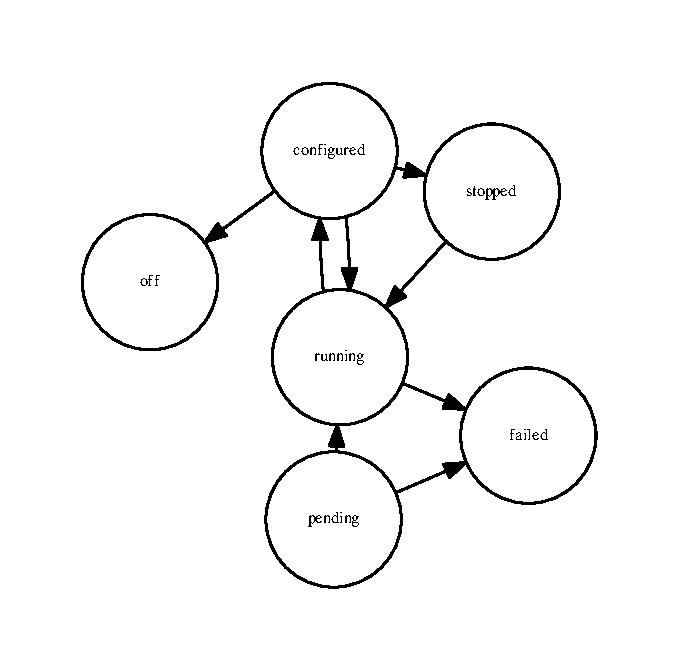
\includegraphics{graphviz-efdf49fbb74513f9f59ebf60f051a790e117d45c.pdf}

\item[{\code{AlterVM}}] \leavevmode\begin{quote}\begin{description}
\item[{parameter 0}] \leavevmode
\code{infId}: integer

\item[{parameter 1}] \leavevmode
\code{vmId}: string

\item[{parameter 2}] \leavevmode
\code{radl}: string

\item[{parameter 3}] \leavevmode
\code{auth}: array of structs

\item[{ok response}] \leavevmode
{[}true, struct(\code{info}: string, \code{cloud}: string, \code{state}: string){]}

\item[{fail response}] \leavevmode
{[}false, \code{error}: string{]}

\end{description}\end{quote}

Change the features of the virtual machine with ID \code{vmId} in the
infrastructure with with ID \code{infId}, specified by the RADL \code{radl}.
Return a struct with information about the virtual machine, like
{\hyperref[xmlrpc:getvminfo-xmlrpc]{\emph{GetVMInfo}}}.

\item[{\code{DestroyInfrastructure}}] \leavevmode\begin{quote}\begin{description}
\item[{parameter 0}] \leavevmode
\code{infId}: integer

\item[{parameter 1}] \leavevmode
\code{auth}: array of structs

\item[{ok response}] \leavevmode
{[}true, string of length zero{]}

\item[{fail response}] \leavevmode
{[}false, \code{error}: string{]}

\end{description}\end{quote}

Undeploy all the virtual machines associated to the infrastructure with ID
\code{infId}.

\end{description}
\phantomsection\label{xmlrpc:addresource-xmlrpc}\begin{description}
\item[{\code{AddResource}}] \leavevmode\begin{quote}\begin{description}
\item[{parameter 0}] \leavevmode
\code{infId}: integer

\item[{parameter 1}] \leavevmode
\code{radl}: string

\item[{parameter 2}] \leavevmode
\code{auth}: array of structs

\item[{ok response}] \leavevmode
{[}true, \code{infId}: integer{]}

\item[{fail response}] \leavevmode
{[}false, \code{error}: string{]}

\end{description}\end{quote}

Add the resources specified in \code{radl} to the infrastructure with ID
\code{infId}. The \code{deploy} instructions in the \code{radl} must refer to
\emph{systems} already defined. If all the \emph{systems} defined in \code{radl} are
new, they will be added. Otherwise the new \emph{systems} defined will be
ignored.

\item[{\code{RemoveResource}}] \leavevmode\begin{quote}\begin{description}
\item[{parameter 0}] \leavevmode
\code{infId}: integer

\item[{parameter 1}] \leavevmode
\code{vmIds}: string

\item[{parameter 2}] \leavevmode
\code{auth}: array of structs

\item[{ok response}] \leavevmode
{[}true, \code{infId}: integer{]}

\item[{fail response}] \leavevmode
{[}false, \code{error}: string{]}

\end{description}\end{quote}

Updeploy the virtual machines with IDs in \code{vmIds} associated to the
infrastructure with ID \code{infId}. The different virtual machine IDs in
\code{vmIds} are separated by commas.

\end{description}
\phantomsection\label{xmlrpc:stopinfrastructure-xmlrpc}\begin{description}
\item[{\code{StopInfrastructure}}] \leavevmode\begin{quote}\begin{description}
\item[{parameter 0}] \leavevmode
\code{infId}: integer

\item[{parameter 1}] \leavevmode
\code{auth}: array of structs

\item[{ok response}] \leavevmode
{[}true, string of length zero{]}

\item[{fail response}] \leavevmode
{[}false, \code{error}: string{]}

\end{description}\end{quote}

Stop (but do not undeploy) all the virtual machines associated to the
infrastructure with ID \code{infId}. They can resume by
{\hyperref[xmlrpc:startinfrastructure-xmlrpc]{\emph{StartInfrastructure}}}.

\end{description}
\phantomsection\label{xmlrpc:startinfrastructure-xmlrpc}\begin{description}
\item[{\code{StartInfrastructure}}] \leavevmode\begin{quote}\begin{description}
\item[{parameter 0}] \leavevmode
\code{infId}: integer

\item[{parameter 1}] \leavevmode
\code{auth}: array of structs

\item[{ok response}] \leavevmode
{[}true, string of length zero{]}

\item[{fail response}] \leavevmode
{[}false, \code{error}: string{]}

\end{description}\end{quote}

Resume all the virtual machines associated to the
infrastructure with ID \code{infId}, previously stopped by
{\hyperref[xmlrpc:stopinfrastructure-xmlrpc]{\emph{StopInfrastructure}}}.

\end{description}
\phantomsection\label{xmlrpc:reconfigure-xmlrpc}\begin{description}
\item[{\code{Reconfigure}}] \leavevmode\begin{quote}\begin{description}
\item[{parameter 0}] \leavevmode
\code{infId}: integer

\item[{parameter 1}] \leavevmode
\code{radl}: string

\item[{parameter 2}] \leavevmode
\code{auth}: array of structs

\item[{ok response}] \leavevmode
{[}true, string of length zero{]}

\item[{fail response}] \leavevmode
{[}false, \code{error}: string{]}

\end{description}\end{quote}

Update the infrastructure with ID \code{infId} using the \emph{configuration
sections} in the RADL \code{radl}. Some virtual machines associated to the
infrastructure may be reconfigured.

\end{description}


\chapter{IM REST API}
\label{REST::doc}\label{REST:im-rest-api}
Optionally, IM Service can be accessed through a REST(ful) API. The port number
and the security settings are controlled by the options listed in
{\hyperref[manual:options-rest]{\emph{REST API}}}.

Every HTTP request must be companied by the header \code{AUTHORIZATION} with
the content of the \emph{auth-file}, but the lines separated with
``\textbackslash{}n'' instead. If the content cannot be parsed successfully, or the user and
password are not valid, it is returned the HTTP error code 401.

Next table summaries the resources and the HTTP methods available.

\begin{tabulary}{\linewidth}{|L|L|L|L|}
\hline
\textsf{\relax 
HTTP method
} & \textsf{\relax 
/infrastructure
} & \textsf{\relax 
/inf/\textless{}infId\textgreater{}
} & \textsf{\relax 
/vms/\textless{}infId\textgreater{}/\textless{}vmId\textgreater{}
}\\
\hline
\textbf{GET}
 & 
\textbf{List} the
infrastructure
IDs.
 & 
\textbf{List} the
virtual machines
in the
infrastructure
\code{infId}
 & 
\textbf{Get} information
associated to the
virtual machine
\code{vmId} in \code{infId}.
\\
\hline
\textbf{POST}
 & 
\textbf{Create} a new
infrastructure
based on the RADL
posted.
 & 
\textbf{Create} a new
virtual machine
based on the RADL
posted.
 & \\
\hline
\textbf{PUT}
 &  & 
\textbf{Stop},
\textbf{start} or
\textbf{reconfigure}
the
infrastructure.
 & 
\textbf{Modify} the virtual
machine based on the
RADL posted.
\\
\hline
\textbf{DELETE}
 &  & 
\textbf{Undeploy} all
the virtual
machine in the
infrastructure.
 & 
\textbf{Undeploy} the
virtual machine.
\\
\hline\end{tabulary}

\begin{description}
\item[{GET \code{http://imserver.com/infrastructure}}] \leavevmode\begin{quote}\begin{description}
\item[{Content-type}] \leavevmode
text/uri-list

\item[{ok response}] \leavevmode
200 OK

\item[{fail response}] \leavevmode
409

\end{description}\end{quote}

Return a list of URIs referencing the infrastructures associated to the IM
user.

\item[{POST \code{http://imserver.com/infrastructure}}] \leavevmode\begin{quote}\begin{description}
\item[{body}] \leavevmode
\code{RADL document}

\item[{Content-type}] \leavevmode
text/uri-list

\item[{ok response}] \leavevmode
200 OK

\item[{fail response}] \leavevmode
409

\end{description}\end{quote}

Create and configure an infrastructure with the requirements specified in
the RADL document of the body contents. If success, it is returned the
URI of the new infrastructure.

\item[{GET \code{http://imserver.com/inf/\textless{}infId\textgreater{}}}] \leavevmode\begin{quote}\begin{description}
\item[{Content-type}] \leavevmode
application/json

\item[{ok response}] \leavevmode
200 OK

\item[{fail response}] \leavevmode
409

\end{description}\end{quote}
\begin{description}
\item[{Return a JSON object with two elements:}] \leavevmode\begin{itemize}
\item {} 
vm\_list: list of URIs referencing the virtual machines associated to the

\end{itemize}
\begin{quote}

infrastructure with ID \code{infId}.
\end{quote}
\begin{itemize}
\item {} 
cont\_out: contextualization message.

\end{itemize}

\end{description}

\item[{POST \code{http://imserver.com/inf/\textless{}infId\textgreater{}}}] \leavevmode\begin{quote}\begin{description}
\item[{body}] \leavevmode
\code{RADL document}

\item[{Content-type}] \leavevmode
text/uri-list

\item[{ok response}] \leavevmode
200 OK

\item[{fail response}] \leavevmode
409

\end{description}\end{quote}

Add the resources specified in the body contents to the infrastructure with ID
\code{infId}. The RADL restrictions are the same as in
{\hyperref[xmlrpc:addresource-xmlrpc]{\emph{RPC-XML AddResource}}}. If success, it is returned
a list of URIs of the new virtual machines.

\item[{PUT \code{http://imserver.com/inf/\textless{}infId\textgreater{}}}] \leavevmode\begin{quote}\begin{description}
\item[{input fields}] \leavevmode
\code{op}, \code{radl} (compulsory if \code{op} is \code{reconfigure})

\item[{Content-type}] \leavevmode
text/uri-list

\item[{ok response}] \leavevmode
200 OK

\item[{fail response}] \leavevmode
409

\end{description}\end{quote}

Perform an action on the infrastructure with ID \code{infID} indicated by the
value of \code{op}:
\begin{itemize}
\item {} 
\code{stop}: stop (but do not undeploy) all the virtual machines in the
infrastructure.

\item {} 
\code{start}: resume all the virtual machines in the infrastructure.

\item {} 
\code{reconfigure}: update the configuration of the infrastructure as
indicated in \code{radl}. The RADL restrictions are the same as in
{\hyperref[xmlrpc:reconfigure-xmlrpc]{\emph{RPC-XML Reconfigure}}}.

\end{itemize}

\item[{DELETE \code{http://imserver.com/inf/\textless{}infId\textgreater{}}}] \leavevmode\begin{quote}\begin{description}
\item[{ok response}] \leavevmode
200 OK

\item[{fail response}] \leavevmode
409

\end{description}\end{quote}

Undeploy the virtual machines associated to the infrastructure with ID
\code{infId}.

\item[{GET \code{http://imserver.com/vms/\textless{}infId\textgreater{}/\textless{}vmId\textgreater{}}}] \leavevmode\begin{quote}\begin{description}
\item[{Content-type}] \leavevmode
application/json

\item[{ok response}] \leavevmode
200 OK

\item[{fail response}] \leavevmode
409

\end{description}\end{quote}

Return information about the virtual machine with ID \code{vmId} associated to
the infrastructure with ID \code{infId}. See the details of the output in
{\hyperref[xmlrpc:getvminfo-xmlrpc]{\emph{GetVMInfo}}}.

\item[{PUT \code{http://imserver.com/vms/\textless{}infId\textgreater{}/\textless{}vmId\textgreater{}}}] \leavevmode\begin{quote}\begin{description}
\item[{body}] \leavevmode
\code{RADL document}

\item[{ok response}] \leavevmode
200 OK

\item[{fail response}] \leavevmode
409

\end{description}\end{quote}

Change the features of the virtual machine with ID \code{vmId} in the
infrastructure with with ID \code{infId}, specified by the RADL document specified
in the body contents.

\item[{DELETE \code{http://imserver.com/vms/\textless{}infId\textgreater{}/\textless{}vmId\textgreater{}}}] \leavevmode\begin{quote}\begin{description}
\item[{ok response}] \leavevmode
200 OK

\item[{fail response}] \leavevmode
409

\end{description}\end{quote}

Undeploy the virtual machine with ID \code{vmId} associated to the
infrastructure with ID \code{infId}.

\end{description}


\chapter{Indices and tables}
\label{index:indices-and-tables}\begin{itemize}
\item {} 
\emph{genindex}

\end{itemize}



\renewcommand{\indexname}{Index}
\printindex
\end{document}
